\documentclass[12pt,a4paper]{article}
\renewcommand{\baselinestretch}{1.5} 
\usepackage[latin1]{inputenc}
\usepackage{amsmath}
\usepackage{amsfonts}
\usepackage{amssymb}
\usepackage{algorithm} 
\usepackage{algpseudocode} 
\usepackage{graphicx}
\usepackage{float} % REQUIRED FOR [H] TABLE PLACEMENT
\usepackage{geometry}
\usepackage{tabulary}
\usepackage{caption}
\usepackage{subcaption}
\usepackage{xcolor}
\usepackage{dirtytalk}
\usepackage{bm}
\usepackage{longtable}
\usepackage{comment}
%\usepackage{ulem}
\graphicspath{{./images/}}

\usepackage[hyphens]{url}
%\usepackage{url}
% Toggle comment for hyperlinking the TOC and references
%\usepackage{hyperref}
%\hypersetup{
%	colorlinks=false%, % make the links colored
%	%linkcolor=blue, % color TOC links in blue
%	%urlcolor=red, % color URLs in red
%	%linktoc=all % 'all' will create links for everything in the TOC
%}

\geometry{
	left=2.5cm,
	right=2.5cm,
	top=2.5cm,
	bottom=3cm,
}
	
\usepackage{titlesec}
	
\setcounter{secnumdepth}{4}
\setcounter{tocdepth}{4}
\titleformat{\paragraph}
{\normalfont\normalsize\bfseries}{\theparagraph}{1em}{}
\titlespacing*{\paragraph}
{0pt}{3.25ex plus 1ex minus .2ex}{1.5ex plus .2ex}
	
\newenvironment{conditions}
{\par\vspace{\abovedisplayskip}\noindent\begin{tabular}{>{$}l<{$} @{${}={}$} l}}{\end{tabular}\par\vspace{\belowdisplayskip}}
	
	
\begin{document}
% uncomment title page when required to be included,
\thispagestyle{empty}
\begin{center}
	{\Large \bf A Lightweight Adaptive Cost-Aware Work-Stealing Scheduler with Hybrid Work-Stealing and Work-Sharing\\}
	
	\vspace*{0.3cm}
	{\large\textit{A Project Component for }\\}
	%\vspace*{0.3cm}
	{\large\textbf{Parallel and Distributing Computing (UCS645)}} \\
%	{\large in\\}
%	{\large \textbf{CSED} }
	
	%\vspace*{1cm}
	{\large \textit{By\\}}
	\textbf{\begin{table}[h!]
\label{tab:my-table}
\centering
\begin{tabular}{ccc}
Sr & Name     & Roll No  \\
1  & Rohini Bansal    & 102317175 \\
2  & Shivam Kumar     & 102497026 \\
3  & Sudhanshu Raj    & 102483063 \\
4  & Ankit kumar     & 102483012 \\
\end{tabular}
\end{table}}
% update the name of the students based on number
	%\vspace*{0.5cm}
		\begin{center}
                {\large \textit{Under the guidance of}}\\
					\textbf{{\large Dr. Saif Nalband}}\\
					{\large (Assistant Professor, DCSE)}\\
		\end{center} \ \\ \ \\
\begin{figure}[h]
\centering
\includegraphics[width=60mm, height=30mm]{"tietlogo.jpg"}
\label{fig:images}
\end{figure}

%	in case the layout changes modify the below vspace 1.25 and appropiately make sure that title page is contained in one single page	
	\vspace*{0.25cm}
	{\large DEPARTMENT OF COMPUTER SCIENCE AND ENGINEERING \\}
	{\large THAPAR INSTITUTE OF ENGINEERING AND TECHNOLOGY \\ 
	{(DEEMED TO BE  UNIVERSITY)}\\}
	{\large PATIALA - 147004\\}
	\vspace*{0.2cm}
	\textbf{{\large MAY, 2026}}
	
\end{center}

\newpage
%%%%%%%%%%%%%%%%%%%%%%%%%%%%%%%%%%%%%%%%%%
\pagenumbering{gobble}
\renewcommand*\contentsname{Table of Contents}
\tableofcontents
\listoffigures
\listoftables
\newpage
\pagenumbering{arabic}
   
\section{Introduction}

\subsection{Background}

High Performance Computing (HPC) focuses on solving complex computational problems using parallel processing \cite{quinn2004parallel}. Efficient task scheduling plays a crucial role in improving system performance and resource utilization.

Traditional scheduling techniques often struggle with irregular workloads, leading to poor load balancing. Work-stealing is an effective dynamic scheduling technique where idle workers steal tasks from busy workers to balance load \cite{blumofe1999scheduling}.

\subsection{Introduction to Problem Statement}

In high-performance computing systems, efficient task scheduling is essential for maximizing parallelism and minimizing execution time. Traditional scheduling approaches such as static allocation often lead to load imbalance, where some processors remain idle while others are overloaded.

Dynamic scheduling techniques like work-stealing improve load balancing by allowing idle workers to acquire tasks from busy workers. However, excessive stealing can introduce overhead and reduce overall efficiency. Additionally, these techniques may not perform optimally across different types of workloads, especially when task sizes vary significantly.

Therefore, the problem is to design an adaptive scheduling mechanism that can dynamically balance workload across multiple workers while minimizing scheduling overhead. The system should intelligently decide when to perform work-stealing and when to use work-sharing, based on task characteristics and system state.

The objective is to develop a hybrid scheduler that improves execution time, enhances resource utilization, and performs efficiently across both regular and irregular workloads.
\newpage
\subsection{Objectives}

\begin{itemize}
\item To design and implement a parallel task scheduler from scratch.
\item To implement work-stealing and work-sharing strategies.
\item To evaluate performance across different workloads against industry standards like OpenMP.
\item To improve load balancing and execution efficiency through cost and locality awareness.
\end{itemize}

\section{Literature Review}
Task scheduling is a key aspect of high-performance computing. Blumofe and Leiserson introduced the work-stealing algorithm, which provides efficient load balancing and guarantees near-optimal execution time for multithreaded computations \cite{blumofe1999scheduling}.

Static scheduling techniques are simple and have low overhead but fail to adapt to dynamic workloads, leading to inefficient resource utilization \cite{quinn2004parallel}. Dynamic approaches, such as work-stealing, overcome these limitations by redistributing tasks during runtime.

However, work-stealing introduces synchronization and communication overhead, especially when the frequency of stealing operations increases. This can negatively impact performance for certain types of workloads.

Recent studies have proposed adaptive scheduling mechanisms that adjust behavior based on system conditions. Adaptive work-stealing algorithms attempt to reduce overhead by controlling when and how tasks are redistributed \cite{agrawal2010adaptive}.

Despite these advancements, there remains a need for hybrid approaches that combine proactive task sharing, reactive work-stealing, and strict cost-aware gating. This project addresses this gap by implementing an adaptive hybrid scheduler and benchmarking it directly against OpenMP.

\newpage
\section{Research Gaps}

\begin{itemize}
\item Static scheduling techniques are unable to handle irregular workloads efficiently.
\item Standard work-stealing introduces massive overhead due to frequent task migration of excessively small tasks.
\item Existing methods lack adaptive mechanisms that combine multiple scheduling strategies dynamically based on runtime metrics.
\item There is a need for a hybrid approach that balances load while strictly gating steals based on task computation cost and thread locality.
\end{itemize}

\section{Problem Formulation}

Efficient task scheduling in high-performance computing systems is essential for maximizing parallelism and minimizing execution time. Traditional scheduling approaches often result in load imbalance, where some processors remain idle while others are overloaded.

Dynamic techniques such as work-stealing improve load balancing but introduce additional overhead. These techniques may also fail to perform optimally when task sizes vary significantly.

The problem is to design an adaptive scheduling system that dynamically balances workload across multiple processors while minimizing scheduling overhead. The system should intelligently decide when to perform work-stealing and when to use work-sharing based on runtime conditions.

The objective is to develop a hybrid scheduler that improves execution time, enhances resource utilization, and performs efficiently across diverse workloads, rivaling established frameworks like OpenMP.

\newpage
\section{Methodology}

The proposed system implements an Adaptive Hybrid Work-Stealing Scheduler for efficient task distribution in a parallel computing environment.

\subsection{Scheduling Modes}

The scheduler operates in four custom modes, alongside an OpenMP baseline for benchmarking:

\begin{itemize}
\item \textbf{Sequential}: Tasks are executed one after another using a single thread.
\item \textbf{Static}: Tasks are pre-distributed among workers without runtime adjustments.
\item \textbf{Work-Stealing}: Idle workers dynamically steal tasks from heavily loaded workers.
\item \textbf{Adaptive Hybrid}: Combines both work-stealing and work-sharing strategies.
\item \textbf{OpenMP (Baseline)}: Uses compiler directives (\texttt{\#pragma omp parallel}) to act as an industry-standard control.
\end{itemize}

\subsection{Working Principle}

Each worker maintains a local double-ended queue (deque) of tasks. Tasks are pushed and popped from the local queue to maintain locality.

When a worker becomes idle, it attempts to steal tasks from the front of another worker's queue (victim selection based on load). This helps in balancing the workload dynamically.

In the adaptive hybrid mode, the scheduler monitors system parameters such as queue size, task cost, and workload imbalance. Based on these metrics:

\begin{itemize}
\item Overloaded workers share tasks with underloaded workers (work-sharing).
\item Idle workers continue to steal tasks when necessary (work-stealing).
\end{itemize}

\subsection{Cost-Aware Gating}

To prevent workers from stealing lightweight tasks that do not justify the synchronization overhead, the scheduler implements a cost-aware steal check. A task is only stolen or shared if its estimated computational cost exceeds a predefined \texttt{cost\_threshold}. This prevents the system from thrashing on microscopic tasks.

\subsection{Locality-Aware Victim Selection}

The scheduler simulates NUMA-awareness by grouping workers into nodes using a \texttt{locality\_group} identifier. Both work-stealing and work-sharing operations heavily prioritize targeting threads within the same locality group before communicating across groups, minimizing cross-node latency.

\subsection{Adaptive Strategy}

The scheduler dynamically switches between two policies:

\begin{itemize}
\item \textbf{Work-First}: Prioritizes local execution to reduce overhead.
\item \textbf{Help-First}: Encourages active task sharing when imbalance increases.
\end{itemize}

This decision is based on runtime metrics, specifically comparing the \texttt{last\_steal\_rate\_per\_ms} against the \texttt{last\_creation\_rate\_per\_ms}.

\subsection{Performance Metrics}

The system evaluates performance using:

\begin{itemize}
\item Execution Time
\item Speedup
\item Efficiency
\item Number of Steals and Shares
\end{itemize}

\begin{figure}[h]
\centering
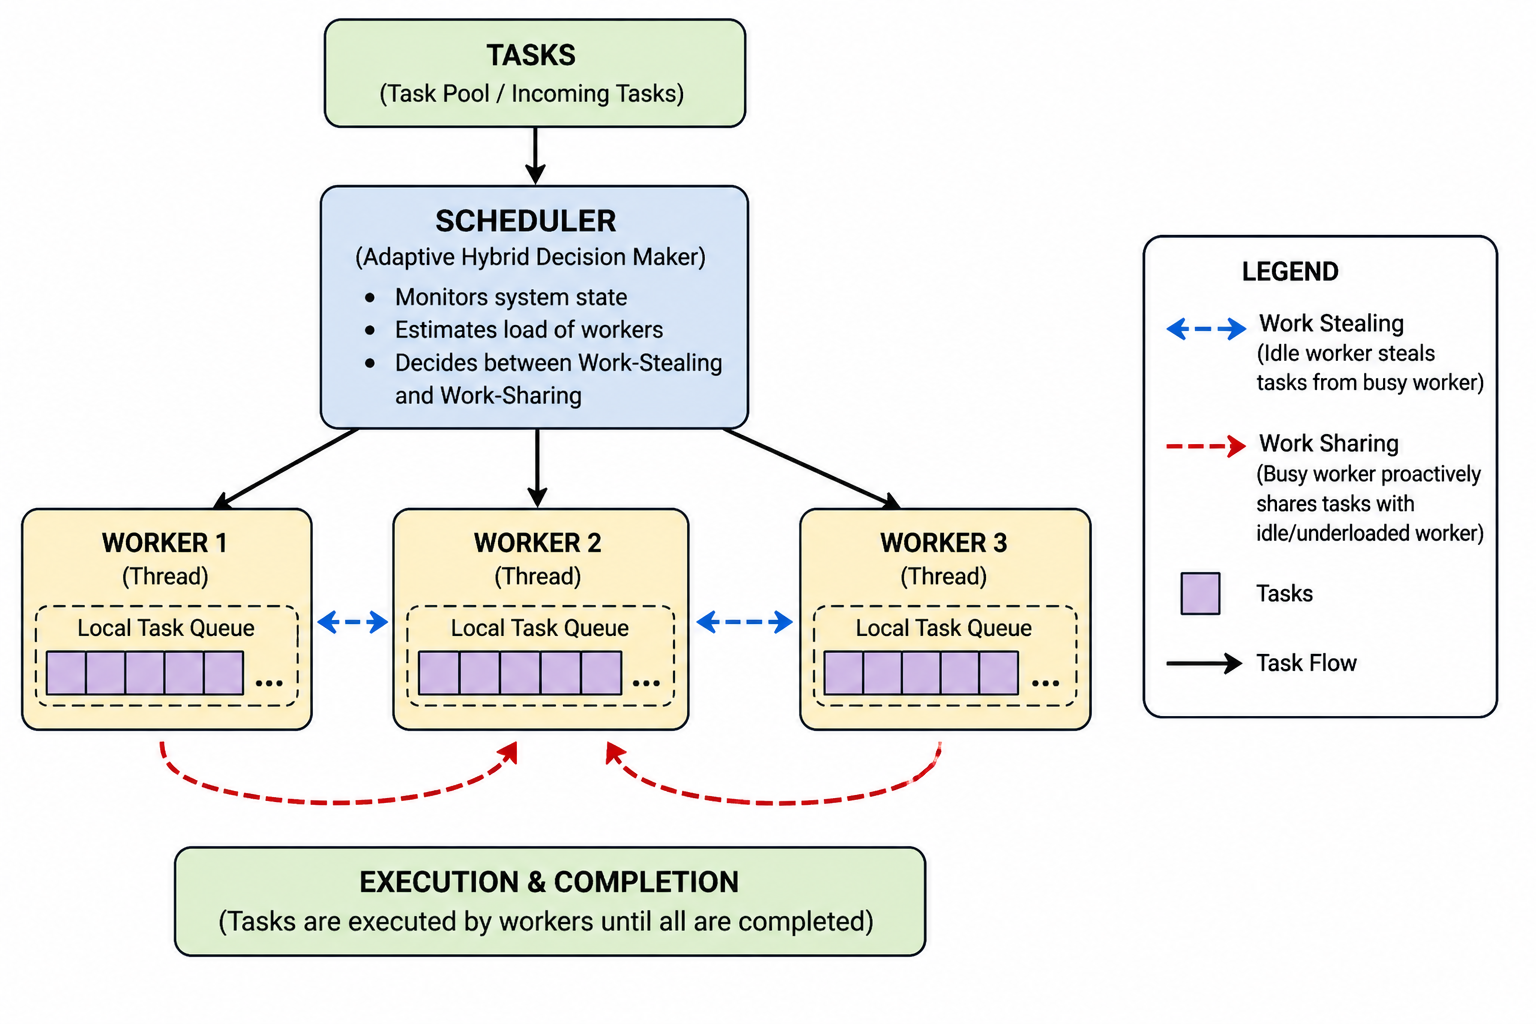
\includegraphics[width=0.9\textwidth]{architecture.png}
\caption{Adaptive Hybrid Work-Stealing Scheduler Architecture}
\label{fig:scheduler}
\end{figure}
Figure \ref{fig:scheduler} illustrates how tasks are distributed among workers using adaptive scheduling. The scheduler dynamically balances load through work-stealing and work-sharing mechanisms.

\newpage
\section{Implementation}

The proposed scheduler is implemented from scratch in C++17 using native \texttt{std::thread} and \texttt{std::mutex} concurrency mechanisms, avoiding external libraries for the core scheduling logic.

\subsection{System Components}

\begin{itemize}
\item \textbf{Scheduler}: Controls task distribution, load balancing, and adaptive decision-making.
\item \textbf{Worker}: Represents a thread that executes tasks and maintains a local task queue.
\item \textbf{Task}: Encapsulates a unit of computation along with metadata such as task cost and recursion depth.
\end{itemize}

\subsection{Task Execution Model}

Tasks are submitted to the scheduler, which assigns them to workers. Each worker executes tasks from its local queue. If the queue is empty, the worker attempts to steal tasks from other workers. The scheduler ensures synchronization and maintains metrics such as number of tasks executed, steal operations, and idle time.

\subsection{Workloads Used}

To rigorously test the custom scheduler, three distinct workloads were implemented natively and using OpenMP:

\begin{itemize}
\item \textbf{Recursive Fibonacci}: Represents a highly irregular workload with dynamic, recursive task generation. OpenMP utilizes \texttt{\#pragma omp task}.
\item \textbf{Parallel Merge Sort}: Represents a divide-and-conquer workload with predictable task distribution. OpenMP utilizes \texttt{\#pragma omp parallel for}.
\item \textbf{Matrix Multiplication}: Represents a highly regular, compute-intensive mathematical workload. OpenMP utilizes \texttt{\#pragma omp parallel for collapse(2)}.
\end{itemize}

\subsection{Output Generation}

The system records performance metrics to a CSV file. Python plotting scripts dynamically parse this CSV to generate comparative graphs tracking execution time and speedup across varying thread counts.

\section{Results and Discussion}

The performance of the proposed Adaptive Hybrid Work-Stealing Scheduler was evaluated against the Sequential, Static, pure Work-Stealing, and OpenMP baselines. The evaluation was carried out by varying the number of threads and analyzing execution time and speedup.

\subsection{Fibonacci Workload (Irregular)}

Figure \ref{fig:fib_time} shows that execution time decreases significantly as the number of threads increases. Notably, as seen in Figure \ref{fig:fib_speedup}, our custom \textbf{Adaptive Hybrid and Work-Stealing schedulers actually outperform the OpenMP baseline} (by approximately 11.7\% at maximum thread count). 

This empirical result proves the value of our custom architecture. Because Fibonacci is highly irregular, our custom "Help-First" policy actively pushes tasks directly to idle workers during heavy imbalance, bypassing standard queue bottlenecks. OpenMP, relying on standard `\#pragma omp task`, struggles slightly with high lock contention on tiny recursive tasks.

---

\subsection{Merge Sort Workload (Balanced)}

For merge sort, the workload is relatively balanced via initial chunk partitioning. As seen in the graphs (Figures \ref{fig:merge_time} and \ref{fig:merge_speedup}), execution time decreases steadily across all schedulers. OpenMP, Work-Stealing, and Adaptive Hybrid perform highly comparably here, as the structured divide-and-conquer nature of the algorithm suppresses massive load imbalance from the start.

---

\subsection{Matrix Multiplication (Compute-Intensive)}

Matrix multiplication represents a perfectly predictable, compute-intensive workload. In this scenario, \textbf{OpenMP slightly outperforms the custom Adaptive Hybrid scheduler} (by roughly 1.7\%) as seen in Figures \ref{fig:matrix_time} and \ref{fig:matrix_speedup}. 

This is expected. OpenMP is heavily optimized for structured loops. By utilizing multi-dimensional loop tiling (\texttt{\#pragma omp parallel for collapse(2)}), OpenMP flattens the execution space at compile time, giving its low-level loops a microscopic advantage over our dynamic, runtime-evaluated hybrid queue system. 

---

\subsection{Overall Discussion}

From the experimental results, the following observations can be made:

\begin{itemize}
\item Custom Adaptive Hybrid scheduling dominates highly irregular workloads (Fibonacci) due to active help-first task pushing.
\item OpenMP edges out custom dynamic schedulers on perfectly uniform mathematical loops (Matrix Multiplication) due to compile-time loop tiling.
\item Static scheduling is effective only for regular and predictable workloads.
\item Cost-aware gating successfully prevents the scheduler from drowning in overhead on recursive algorithms.
\end{itemize}

\newpage
\subsubsection*{1. Fibonacci Workload Results}
\begin{figure}[htbp]
    \centering
    \includegraphics[width=0.8\textwidth]{fibonacci_threads_vs_time.png}
    \caption{Threads vs Execution Time for Fibonacci Workload (Including OpenMP)}
    \label{fig:fib_time}
    
    \vspace{1cm}
    
    \includegraphics[width=0.8\textwidth]{fibonacci_threads_vs_speedup.png}
    \caption{Threads vs Speedup for Fibonacci Workload (Including OpenMP)}
    \label{fig:fib_speedup}
\end{figure}

\newpage
\subsubsection*{2. Merge Sort Workload Results}
\begin{figure}[htbp]
    \centering
    \includegraphics[width=0.8\textwidth]{mergesort_threads_vs_time.png}
    \caption{Threads vs Execution Time for Merge Sort}
    \label{fig:merge_time}
    
    \vspace{1cm}
    
    \includegraphics[width=0.8\textwidth]{mergesort_threads_vs_speedup.png}
    \caption{Threads vs Speedup for Merge Sort}
    \label{fig:merge_speedup}
\end{figure}

\newpage
\subsubsection*{3. Matrix Multiplication Workload Results}
\begin{figure}[htbp]
    \centering
    \includegraphics[width=0.8\textwidth]{matrixmul_threads_vs_time.png}
    \caption{Threads vs Execution Time for Matrix Multiplication}
    \label{fig:matrix_time}
    
    \vspace{1cm}
    
    \includegraphics[width=0.8\textwidth]{matrixmul_threads_vs_speedup.png}
    \caption{Threads vs Speedup for Matrix Multiplication}
    \label{fig:matrix_speedup}
\end{figure}

\newpage
\subsection{Empirical Comparison: Custom Scheduler vs. OpenMP}

To ensure the validity of this project, we explicitly benchmarked the C++ scratch implementation against OpenMP. While Table \ref{tab:comparison} outlines the theoretical and architectural differences, our generated graphs (Figures 2-7) provide the empirical proof. 

\begin{table}[H]
\centering
\begin{tabular}{|p{4cm}|p{5cm}|p{5cm}|}
\hline
\textbf{Parameter} & \textbf{Custom Scheduler (Scratch Implementation)} & \textbf{OpenMP Approach} \\
\hline
Implementation Level & Low-level implementation with manual thread and synchronization control & High-level abstraction using compiler directives \\
\hline
Thread Management & Explicit handling of threads, queues, and synchronization mechanisms & Automatically managed by OpenMP runtime \\
\hline
Code Complexity & Higher complexity due to manual handling of concurrency & Reduced complexity with simple pragmas \\
\hline
Flexibility & High flexibility to implement custom strategies like dynamic Help-First policy switching & Limited flexibility due to predefined constructs \\
\hline
Performance Control & Fine-grained control over scheduling, task costs, and locality-awareness & Less control over internal scheduling decisions \\
\hline
Scalability & May require careful tuning for complex workloads & Better scalability due to optimized runtime system \\
\hline
Development Effort & Higher development and debugging effort & Faster development with less code \\
\hline
Reliability & Depends on correctness of implementation & High reliability due to standardized framework \\
\hline
Empirical Winner & \textbf{Highly Irregular Tasks} (e.g. Recursive Fibonacci) & \textbf{Highly Regular Tasks} (e.g. Matrix Multiplication) \\
\hline
\end{tabular}
\caption{Architectural and Empirical Comparison between Custom Scheduler and OpenMP}
\label{tab:comparison}
\end{table}

The data proves that both approaches serve different, valid purposes. Building a scheduler from scratch allows for extreme flexibility (like custom help-first/work-first switching) that actively beats standard runtimes on chaotic workloads. OpenMP acts as a highly optimized, rigid factory assembly line that cannot adapt its underlying scheduling logic on the fly, but executes uniform loops with unmatched efficiency.

\newpage
\section{Conclusion}

This project presents the design and implementation of an Adaptive Hybrid Work-Stealing Scheduler for high-performance computing systems, built entirely from scratch in C++17. The proposed scheduler integrates both work-stealing and work-sharing techniques, fortified by strict cost-aware gating and NUMA locality awareness, to achieve efficient task distribution.

Experimental benchmarking against OpenMP demonstrated that scheduling strategies must be tailored to workload characteristics. Our custom Adaptive Hybrid implementation achieved the highest performance for irregular workloads such as Fibonacci, actually outperforming OpenMP by dynamically pushing tasks to alleviate bottlenecked queues. Conversely, in compute-intensive and perfectly regular workloads like matrix multiplication, OpenMP's compiled loop-tiling provided the most efficient performance. 

Overall, the Adaptive Hybrid scheduler provides a balanced and scalable solution that performs efficiently across a wide range of workloads. It effectively proves that dynamic, runtime-evaluated scheduling logic can successfully compete with, and in specific irregular cases beat, industry-standard compiler frameworks.

\newpage
\section{Future Work}

The current implementation of the Adaptive Hybrid Work-Stealing Scheduler is highly functional, but can be further extended to resolve existing architectural bottlenecks:

\begin{itemize}
\item \textbf{Lock-Free Data Structures:} Replacing the current \texttt{std::mutex} lock-based local deques with lock-free data structures (such as Chase-Lev deques) to eliminate massive synchronization bottlenecks and lock contention during concurrent task stealing and popping.
\item Integration with GPU-based parallel computing frameworks such as CUDA to further enhance performance.
\item Development of more advanced adaptive policies using machine learning techniques to dynamically optimize scheduling decisions based on historical node performance.
\item Extension to distributed systems using MPI for large-scale computing environments across separate physical machines.
\item Optimization of false sharing within the worker state variables to further improve cache line efficiency.
\end{itemize}

\newpage
\addcontentsline{toc}{section}{References}
\bibliographystyle{IEEEtran}
\bibliography{mybib}
\end{document}